\begin{figure}[pos=t]
    \centering
    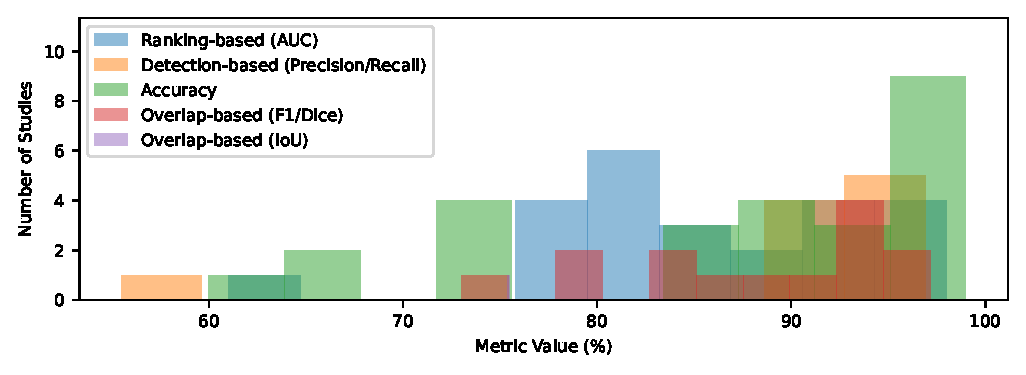
\includegraphics[width=1\linewidth]{histogram_metrics.pdf}
    \caption{Histogram of primary performance metric values across included studies, normalised to a common 0--100 scale and stratified by metric family. Overlap-based metrics (F1/Dice) are distributed broadly across the 40--100 range, with the largest concentration in the 70--80 and 80--90 bins. Accuracy values cluster strongly in the 90--100 bin. Ranking-based AUC values are concentrated in the 80--100 range. The distribution illustrates both the range of reported performance and the heterogeneity of evaluation conventions that prevents direct cross-study comparison.}
    \label{fig:metric_histogram}
\end{figure}
